\documentclass[a4paper,12pt]{article}

\usepackage[top=3cm, bottom=2cm, left=3cm, right=2cm]{geometry}
\usepackage[utf8]{inputenc}
\usepackage[portuguese]{babel}
\usepackage{booktabs}
\usepackage{multirow}
\usepackage{hyperref}
\usepackage{graphicx}
\usepackage{longtable}
\usepackage{verbatim}
\usepackage{url}

\usepackage{morefloats}
\usepackage{float}
\floatstyle{ruled}
\newfloat{program}{thp}{lop}
\floatname{program}{Log}
\newfloat{config}{thp}{lop}
\floatname{config}{Configuração}

\title{Serviços de Rede e de Sistema \\
Exterior Routing }

\author{André Fernandes (ei03107) \and Miguel Gomes (ei07075) \and Pedro Batista (ext10392)}

\begin{document}

\maketitle

\section{Topologia}

Neste trabalho, a topologia de rede foi ligeiramente alterada face à 
proposta no protocolo. No mesmo é proposto uma configuração do protocolo BGP 
que permitisse interligar todas as 6 bancadas do laboratório. 
Em virtude de termos realizado o trabalho isoladamente decidimos apenas 
interligar 4 bancadas (as primeiras três e a sexta).
No entanto, todos os ASs permaneceram compostos por 4 routers interligados pelo 
protocolo OSPF e distribuidos por duas VLANs, à semelhança do trabalho anterior. 

Na figura \ref{fig:topologia} é possível observar a topologia dos ABR da rede,
bem como o seu endereçamento.

\begin{figure}[htp]
	\begin{center}
		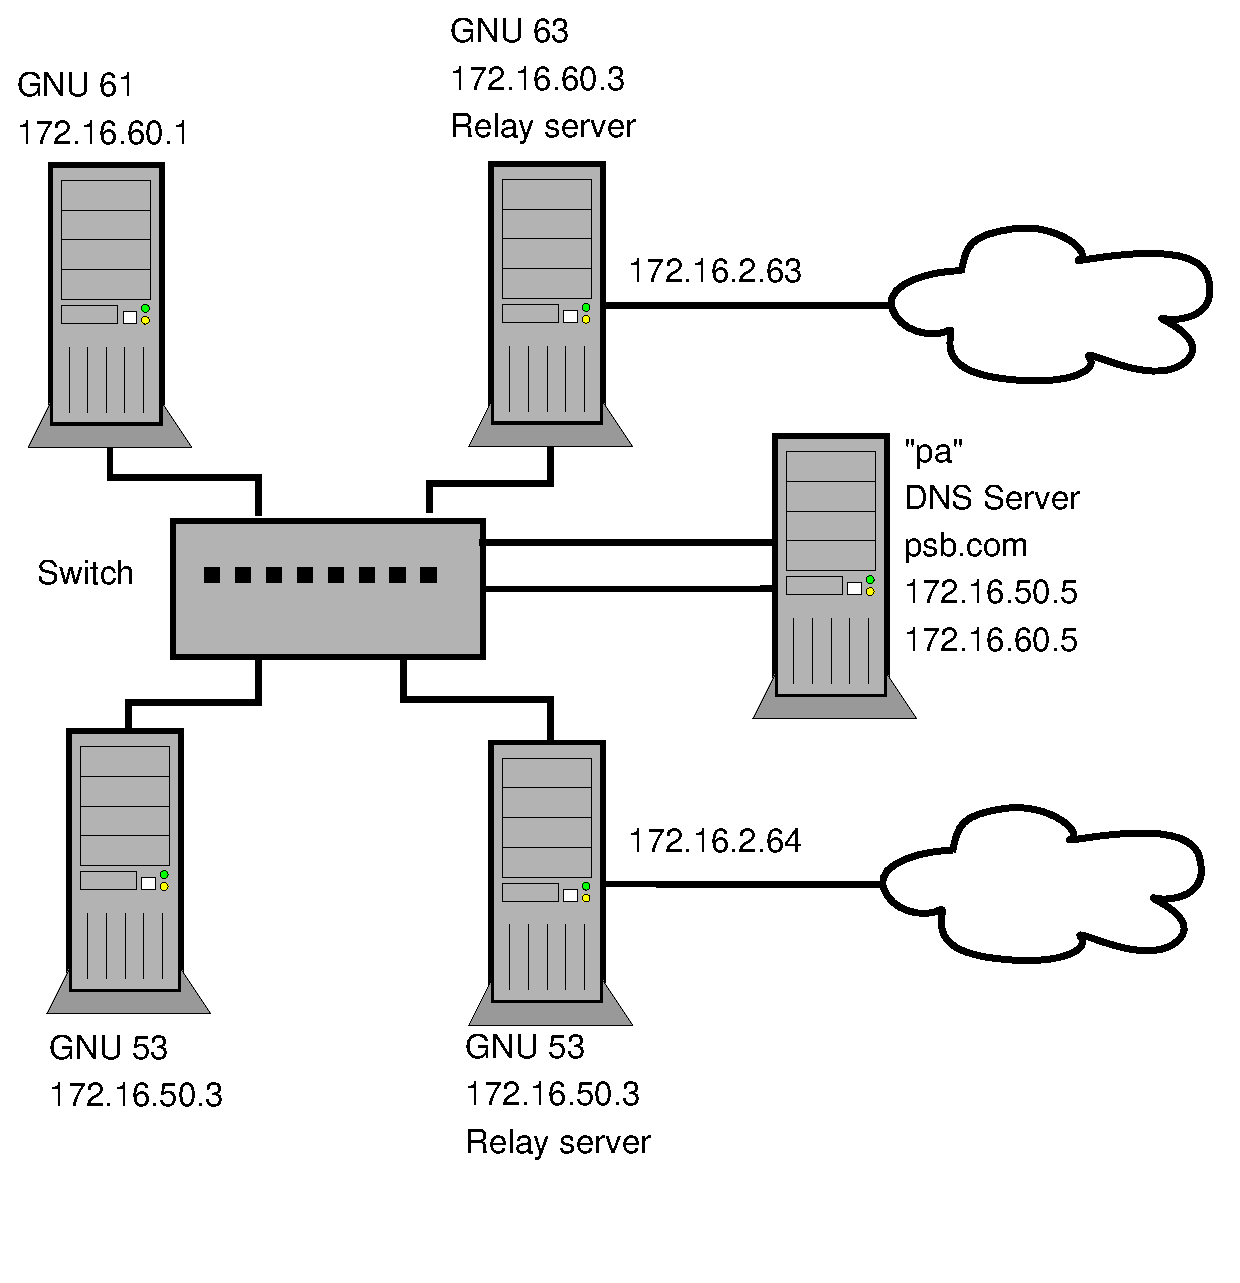
\includegraphics[width=6in]{topologia}
	\end{center}
	\caption{Topologia de rede implementada.}
	\label{fig:topologia}
\end{figure}

\newpage

\section{Cenários}

Após termos configurado a rede tal como descrito anteriormente, estudámos o comportamento 
da rede em dois cenários diferentes. No primeiro cenário foi analizado o comportamento 
da rede quando cada ABR dá a mesma importância aos seus vizinhos directos.
Já no segundo caso, verificámos como é que o protocolo BGP funciona quando atribuímos
importâncias diferentes aos vizinhos directos. Neste caso, cada ABR deu maior
prioridade aos vizinhos com maior número identificador do AS.

\section{Análise de Tráfego}

Em primeiro lugar observou-se o correcto funcionamento do protocolo BGP. 
Sempre que um ABR entrou no sistema, o protocolo BGP permitiu a deteção
dessa nova entrada pelos restantes ABR. E, consequentemente, verificou-se 
a actualização de todas as tabelas de roteamento de todos os ABR.

Após a configuração de toda a rede e tal como os registos do cenário 1 
podem comprovar. Os ABR que estão diagonalmente opostos, dispõem sempre de 
duas rotas entre si com um mesmo custo.

Ainda no cenário 1, podemos verificar que os ABR nunca escolhem a rota mais
longa para ligarem-se aos ABR que são vizinhos directos.

Por último, e como se pode verificar pelos registos do cenário 2,
os ABR dão sempre prioridade às rotas com maior peso. A título de exemplo, o 
ABR do AS003 dá sempre preferência ao ABR da AS006 para os ABR AS003 e AS006.

Os registos das rotas e \verb traceroute  associados a estas afirmações encontram-se
em anexo.

\begin{program}
	\verbatiminput{c1/show_route_as1}
  \caption{Rotas do ABR do AS 001 no primeiro cenário.}
\end{program}

\begin{program}
	\verbatiminput{c1/traceroute_as1}
  \caption{Traceroutes do ABR do AS 001 no primeiro cenário.}
\end{program}

\begin{program}
	\verbatiminput{c1/show_route_as2}
  \caption{Rotas do ABR do AS 002 no primeiro cenário.}
\end{program}

\begin{program}
	\verbatiminput{c1/traceroute_as2}
  \caption{Traceroutes do ABR do AS 002 no primeiro cenário.}
\end{program}

\begin{program}
	\verbatiminput{c1/show_route_as3}
  \caption{Rotas do ABR do AS 003 no primeiro cenário.}
\end{program}

\begin{program}
	\verbatiminput{c1/traceroute_as3}
  \caption{Traceroutes do ABR do AS 003 no primeiro cenário.}
\end{program}

\begin{program}
	\verbatiminput{c1/show_route_as6}
  \caption{Rotas do ABR do AS 006 no primeiro cenário.}
\end{program}

\begin{program}
	\verbatiminput{c1/traceroute_as6}
  \caption{Traceroutes do ABR do AS 006 no primeiro cenário.}
\end{program}

\begin{program}
	\verbatiminput{c3/show_route_as1}
  \caption{Rotas do ABR do AS 001 no segundo cenário.}
\end{program}

\begin{program}
	\verbatiminput{c3/traceroute_as1}
  \caption{Traceroutes do ABR do AS 001 no segundo cenário.}
\end{program}

\begin{program}
	\verbatiminput{c3/show_route_as2}
  \caption{Rotas do ABR do AS 002 no segundo cenário.}
\end{program}

\begin{program}
	\verbatiminput{c3/traceroute_as2}
  \caption{Traceroutes do ABR do AS 002 no segundo cenário.}
\end{program}

\begin{program}
	\verbatiminput{c3/show_route_as3}
  \caption{Rotas do ABR do AS 003 no segundo cenário.}
\end{program}

\begin{program}
	\verbatiminput{c3/traceroute_as3}
  \caption{Traceroutes do ABR do AS 003 no segundo cenário.}
\end{program}

\begin{program}
	\verbatiminput{c3/show_route_as6}
  \caption{Rotas do ABR do AS 006 no segundo cenário.}
\end{program}

\begin{program}
	\verbatiminput{c3/traceroute_as6}
  \caption{Traceroutes do ABR do AS 006 no segundo cenário.}
\end{program}

\begin{config}
	\verbatiminput{conf_bgp/conf}
	\caption{Configurações gerais para todos os ABR.}
\end{config}

\begin{config}
	\verbatiminput{conf_bgp/conf_as001}
	\caption{Configurações BGP para ABR do AS 001.}
\end{config}

\begin{config}
	\verbatiminput{conf_bgp/conf_as002}
	\caption{Configurações BGP para ABR do AS 002.}
\end{config}

\begin{config}
	\verbatiminput{conf_bgp/conf_as003}
	\caption{Configurações BGP para ABR do AS 003.}
\end{config}

\begin{config}
	\verbatiminput{conf_bgp/conf_as006}
	\caption{Configurações BGP para ABR do AS 006.}
\end{config}

\end{document}
